\subsection{Architectures}

\begin{figure}
    \centering
    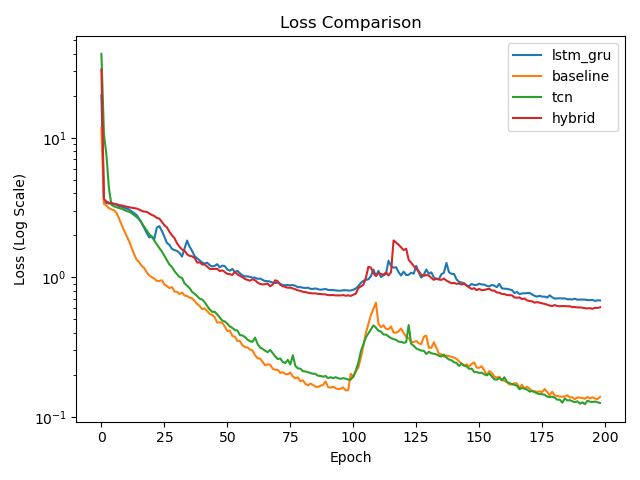
\includegraphics[width=0.8\textwidth]{figures/all_losses.png}
    \caption{Training losses for all architectures.}
\end{figure}

\begin{figure}
    \centering
    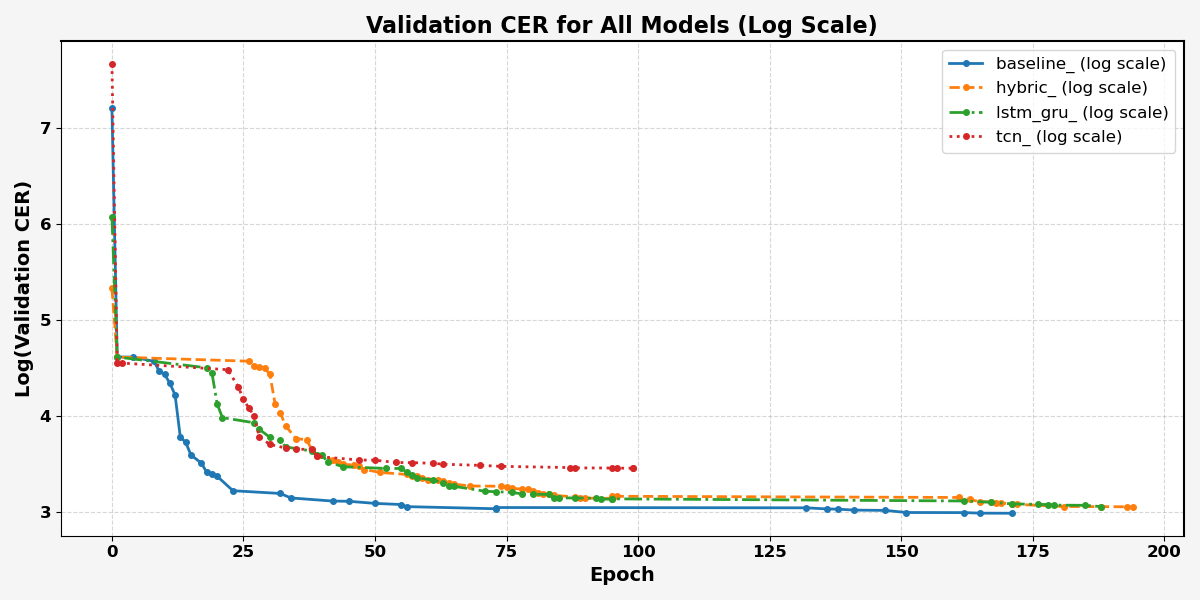
\includegraphics[width=0.8\textwidth]{figures/Val_cer.png}
    \caption{Validation CER for all architectures.}
\end{figure}

\begin{figure}
    \centering
    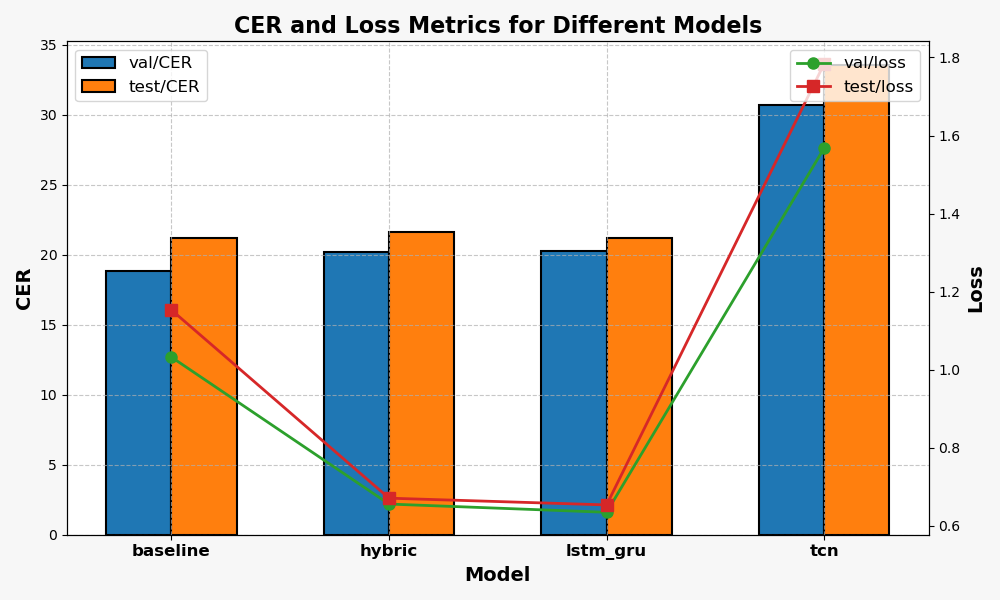
\includegraphics[width=0.8\textwidth]{figures/test.png}
    \caption{Test CER for all architectures.}
\end{figure}

All four neural architectures were trained for a total of $200$ epochs. Due to computational constraints, we partitioned the training into two consecutive phases of $100$ epochs each. We checkpointed each model after the initial $100$ epochs, resuming the second phase of training from these checkpoints. To differentiate clearly between these two training stages, we appended the suffix \texttt{\_200} to denote metrics collected during the second $100$ epochs.

\subsubsection{Baseline (TDSConv) Model.}

The baseline model, adapted directly from Hannun et al., consistently achieved the strongest performance among all architectures tested. Throughout the $200$ epochs, its training loss exhibited a steady, continuous decline, suggesting that the network had not yet reached full convergence. Furthermore, the validation Character Error Rate (CER) similarly reflected persistent improvement, reinforcing the baseline’s effectiveness at generalizing beyond the training set. This ongoing downward trend in both metrics indicates that, given extended training epochs or additional computational resources, the baseline may yield further performance gains. Such strong performance underscores the suitability of Time-Depth Separable convolutions for capturing the underlying patterns present in sEMG signals for keystroke prediction.

\subsubsection{Temporal Convolutional Network (TCN).}

The TCN-based architecture showed promising early training dynamics, characterized by rapid decreases in loss, mirroring the baseline model’s trajectory. We attribute this similarity to the shared convolutional backbone between TCN and TDSConv, allowing both models to efficiently extract local temporal features from sEMG inputs. However, despite the initially impressive loss reduction, TCN began showing signs of overfitting in later training stages. This phenomenon was evident from the plateauing and subsequent slight deterioration in the validation CER, despite continued reductions in the training loss. This discrepancy indicates that the TCN model effectively memorized subtle nuances in the training dataset, but struggled to generalize well to unseen data. The early promise and later challenges of the TCN architecture suggest the need for further regularization techniques, such as dropout or weight decay, to better manage model capacity and enhance generalization.

\subsubsection{LSTM+GRU Model.}

Our recurrent-only approach, composed of stacked LSTM and GRU layers, presented a distinctly different training profile compared to convolutional architectures. Initially, the recurrent model demonstrated slower convergence in terms of loss reduction. Such gradual initial convergence aligns with expectations, as recurrent neural networks typically require extended training periods to effectively learn long-range temporal dependencies. Encouragingly, towards the end of the $200$ epochs, the LSTM+GRU model still exhibited a persistent, albeit slow, decline in both training loss and validation CER, indicating continued learning potential. The ongoing improvements observed at the conclusion of training strongly suggest that the model had not reached its optimal performance and could further benefit from prolonged training or more aggressive optimization strategies.

\subsubsection{Hybrid (TCN+LSTM+GRU) Model.}

The hybrid architecture, intended to leverage the strengths of both convolutional and recurrent structures, exhibited a training profile similar to, though slightly inferior than, the purely recurrent LSTM+GRU approach. Despite early expectations that combining local convolutional feature extraction (via TCN) and global temporal context modeling (via LSTM and GRU layers) might yield superior performance, the observed results did not fully realize these advantages. We hypothesize that introducing convolutional components into a recurrent pipeline increased overall model complexity, thereby posing additional challenges in training optimization. Specifically, the hybrid model might not have fully exploited the richer representations generated by the TCN front end within the available computational resources and training time. Consequently, additional hyperparameter tuning or the introduction of intermediate regularization measures may be necessary to unlock the hybrid model’s full potential.

    
\subsubsection{Summary and Discussion}

In summary, the baseline TDSConv model consistently outperformed our alternative architectures, showcasing a robust and reliable capability to decode keystrokes from sEMG signals. The purely convolutional TCN architecture shared rapid initial convergence characteristics with TDSConv, yet suffered from overfitting later in training. Conversely, the purely recurrent LSTM+GRU model, although slower to converge initially, continued improving through the entirety of training, indicating substantial room for growth with further optimization. Finally, the hybrid TCN+LSTM+GRU model, while theoretically appealing, faced optimization difficulties due to increased complexity and thus did not outperform simpler approaches. Future research directions may explore extended training duration, advanced regularization methods, targeted data augmentation strategies, or further hyperparameter tuning, to better capitalize on the strengths of each proposed model.
